\section{Real-world Scenarios}

\subsection{Real-world Scenarios}
\begin{frame}
	\frametitle{Real-world Scenarios}
	\begin{itemize}
		\setlength\itemsep{1em}
		\item Natural language text: 2.59x faster
		\item DNA sequences: 5.45x faster
		\item Protein sequences 6.88x faster
	\end{itemize}
\end{frame}	

\begin{frame}
	\begin{figure}
		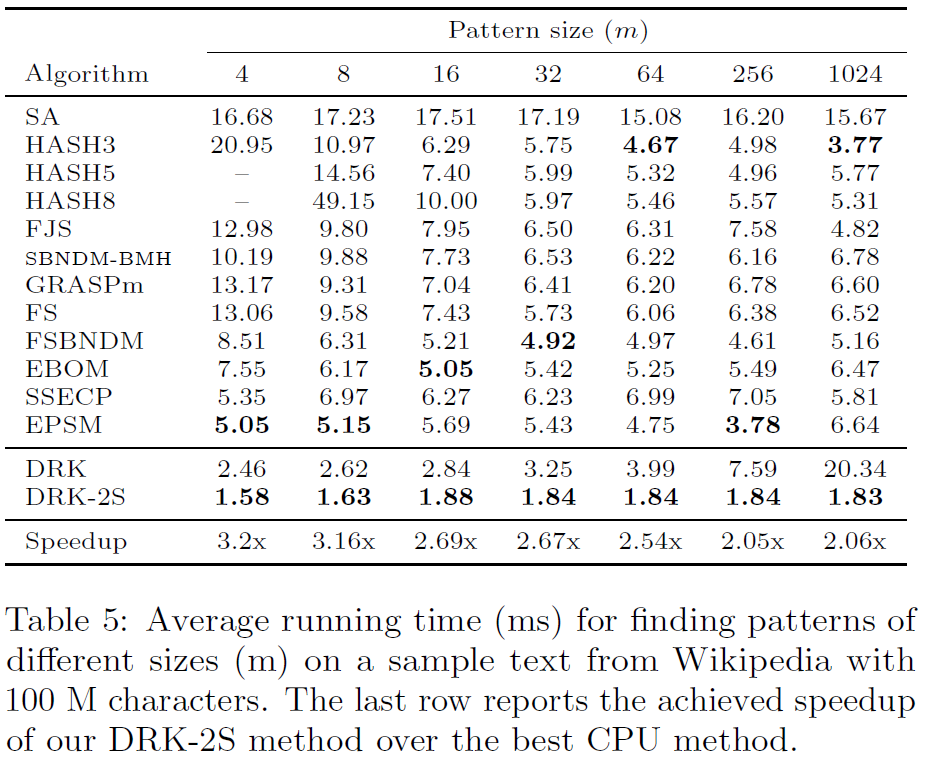
\includegraphics[scale=0.40]{figure/fig-wiki.png}
	\end{figure}
\end{frame}

\begin{frame}
	\begin{figure}
		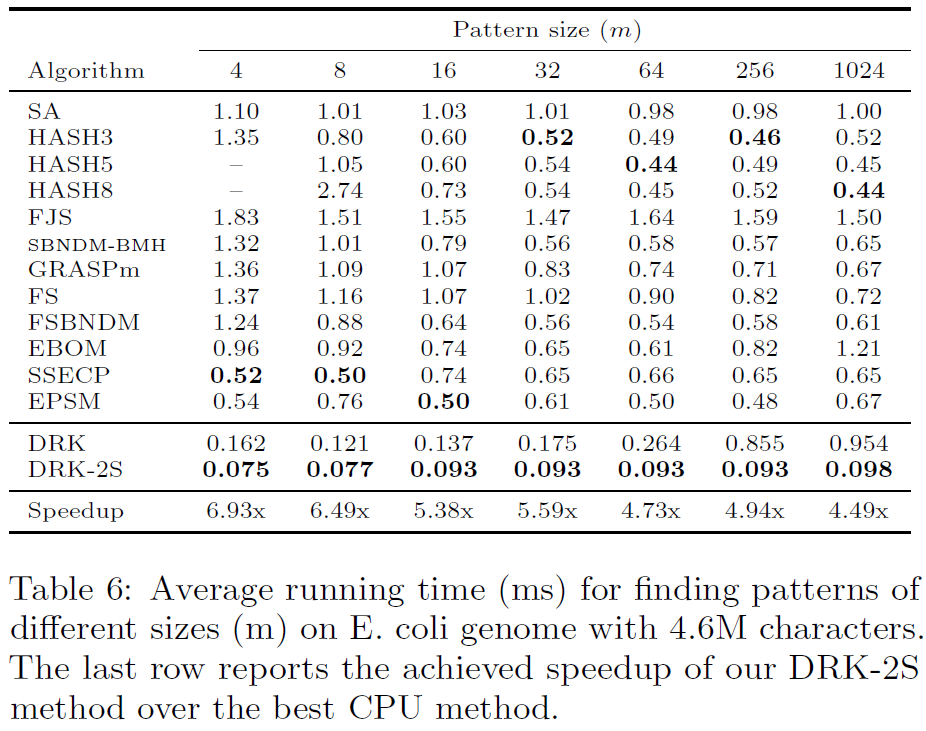
\includegraphics[scale=0.40]{figure/fig-dna.png}
	\end{figure}
\end{frame}

\begin{frame}
	\begin{figure}
		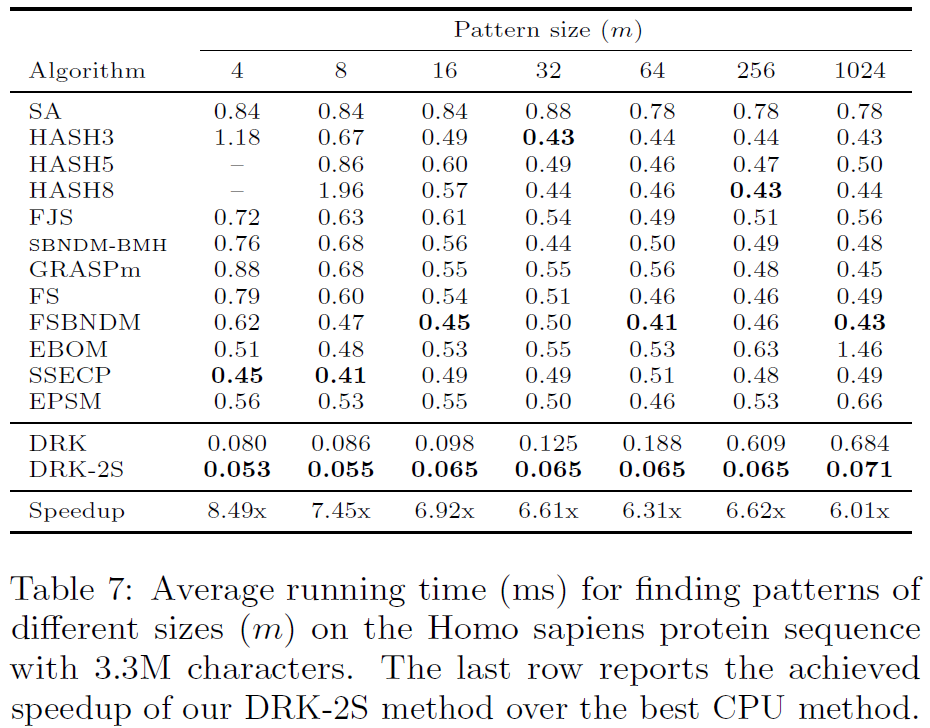
\includegraphics[scale=0.40]{figure/fig-protein.png}
	\end{figure}
\end{frame}

\subsection{False Positives}
\begin{frame}
	\frametitle{False Positives}
	\begin{itemize}
		\setlength\itemsep{1em}
		\item If the chosen prime number is less than 
		$n(n-m+1)^2$, then the probability of error is
		upper-bouded by $2.511 / (n-m+1)$.
		\item We could arbitrarily decrease the false
		positive probability even more by hashing each chunk
		with a different prime number.
	\end{itemize}
\end{frame}


